\documentclass{beamer}
\usetheme{Madrid}
\usepackage{lmodern}
\usepackage{hyperref}
\usepackage{apacite}
\usepackage[utf8]{inputenc}
\usepackage[spanish]{babel}

\usepackage{xcolor}
\setbeamertemplate{background}{\tikz[overlay,remember picture]\node[opacity=0.2]at (current page.center){
\includegraphics[width=13cm]{KL.png}};}
\usepackage{tikz}
\usepackage{kantlipsum}

\setbeamercolor{normal text}{fg=black}

\begin{document}
\colorlet{beamer@blendedblue}{blue!46!green}
\setbeamercolor{normal text}{fg=black}

\setbeamercolor{frametitle}{fg=white, bg=blue!46!green}
\setbeamercolor*{title}{bg=blue!46!green, fg=white}

\setbeamercolor{section in toc}{fg=black}

\author[Juan C. Correa \textcolor{white}{(\url{https://correajc.com}})]{Juan C. Correa, Ph.D.}
\title[Enseñanza basada en reproducibilidad]{Enseñanza basada en reproducibilidad}
\subtitle{Modelado y Simulación de Fenómenos basados en Agentes}
	%\subtitle{}
\institute[]{Fundación Universitaria Konrad Lorenz\\
	\color{blue}\Email  \href{mailto:juanc.correan@konradlorenz.edu.co}{juanc.correan@konradlorenz.edu.co}}
\pgfdeclareimage[height=0.5cm]{KL}{KL}
\logo{\pgfuseimage{KL}}
\setbeamertemplate{caption}[numbered]
\date[Bogotá, Junio-2021]{Curso en: \textbf{T}ecnologías \textbf{R}eproducibles en la \textbf{E}nseñanza de la \textbf{M}etodología y la \textbf{E}stadística}

%\subject{}
\setbeamercolor{background canvas}{bg=white}
%\setbeamertemplate{navigation symbols}{}

\begin{frame}
	\titlepage
\end{frame}

\begin{frame}
\begin{block}{Objetivo del Curso}
\vspace{0.3cm}
Comprender, a través del software \textbf{NetLogo}, los beneficios de adoptar nuevas tecnologías reproducibles para la enseñanza de contenidos metodológicos y estadísticos orientados al modelado y simulación de fenómenos de interés para las ciencias naturales y sociales.
\end{block}
\end{frame}



\begin{frame}
\frametitle{Agenda} 
\tableofcontents
\end{frame}

\section{¿Qué es NetLogo?}
\begin{frame}{¿Qué es NetLogo?}
NetLogo es un lenguaje de programación dentro de un entorno de desarrollo integrado para modelar y simular fenómenos implementando \textbf{agentes inteligentes} \cite{Tisue2004}.
\end{frame}

\subsection{¿Qué es un agente?}
\begin{frame}{¿Qué es un agente?}
Un agente inteligente (en su ``noción débil'') es una entidad no biológica, con las siguientes propiedades: \cite{Wooldridge1995}:
\vspace{0.3cm}
\begin{itemize}
\item \textbf{Autonomía}: Actúan sin la intervención directa de un humano, teniendo cierto grado de control sobre sus propias acciones.
\vspace{0.2cm}
\pause
\item \textbf{Habilidad social}: Interactúan con otros agentes o humanos empleando alguna clase de comunicación.
\vspace{0.2cm}
\pause
\item \textbf{Reactividad}: Perciben el entorno en el que se encuentran (natural y/o virtual) y se adaptan a los cambios que ahí observan.
\vspace{0.2cm}
\pause
\item \textbf{Proactividad}: Son capaces de mostrar conductas orientadas a metas tomando la iniciativa y actuando con anticipación a la ocurrencia de eventos en su entorno.
\end{itemize}
\end{frame}

\begin{frame}{¿Qué es un agente?}
Según \citeauthor{Wooldridge1995} \citeyear{Wooldridge1995} la ``noción fuerte'' de agentes, además de incorporar a la noción débil, asume al agente como un sistema ``que emplea conceptos que se aplican más usualmente a los humanos'' (p. 117); lo que implica que los agentes tienen ``conocimientos'', ``obligaciones'', `intenciones'' o hasta ``emociones''.
    
\end{frame}



\section{Justificación de la herramienta}
\begin{frame}{Justificación de la herramienta}
\tiny{\textcolor{blue}{\url{https://ccl.northwestern.edu/2020/Final\%20Draft.pdf}}}
\begin{figure}
\centering
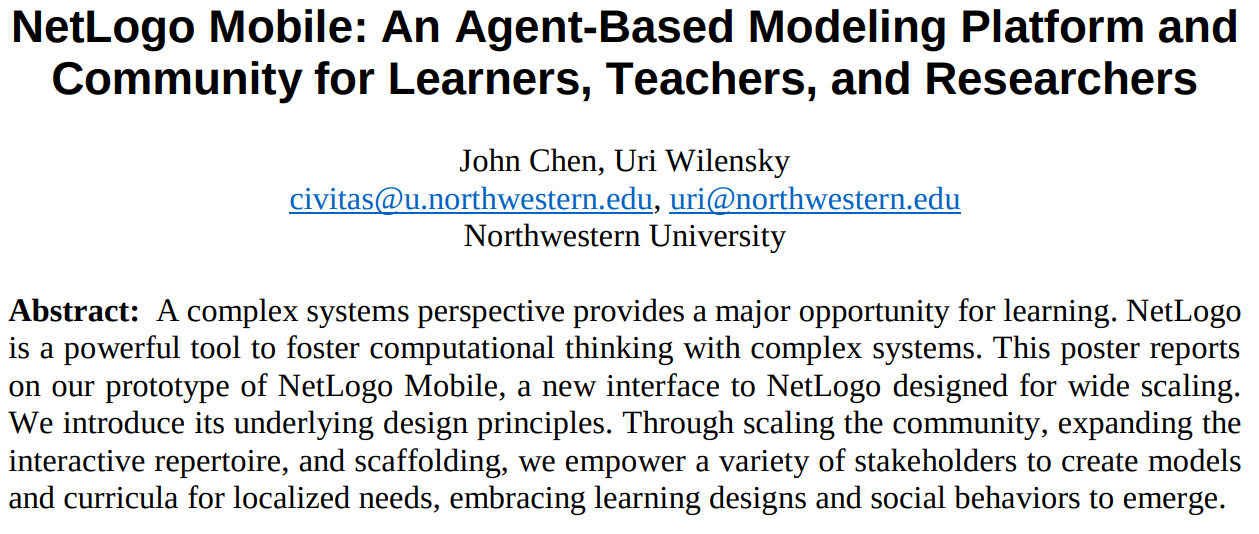
\includegraphics[width=.9\textwidth]{NetlogoJ.png}
\end{figure}
\cite{Chen2020}
\end{frame}

\begin{frame}{Justificación de la Herramienta}
``\textit{Las ideas poderosas son las que pueden usarse como herramientas para pensar durante toda la vida. La idea de un sistema complejo es intrínsecamente poderosa (...) brinda una gran oportunidad para cerrar la brecha cada vez mayor entre la comprensión actual en el mundo académico, la práctica de los profesionales, los hacedores de política y los ciudadanos.}''\\
\cite[p. 2633]{Chen2020}
\end{frame}

\begin{frame}{Justificación de la Herramienta}
En la librería de NetLogo hay muchísimos modelos listos para usar.
\begin{figure}
\centering
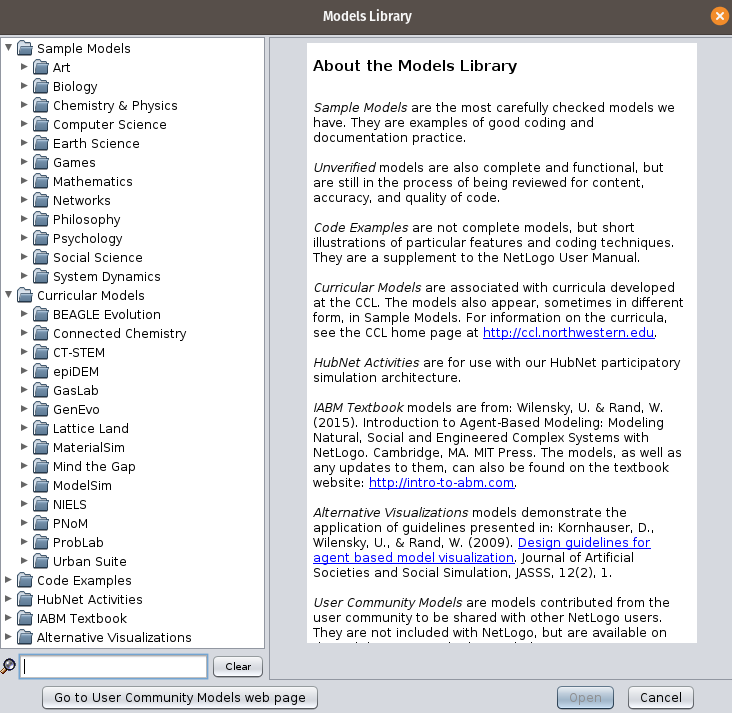
\includegraphics[width=.6\textwidth]{biblioteca.png}
\end{figure}
\end{frame}

\section{Requerimientos Técnicos}
\begin{frame}{Requerimientos Técnicos}
Para seguir el paso a paso de este tutorial, es necesario que usted cuente con un acceso a Internet para visitar la página de Netlogo web  (\textcolor{blue}{\url{http://www.netlogoweb.org/}}) o instalar NetLogo Desktop (\textcolor{blue}{\url{https://ccl.northwestern.edu/netlogo/download.shtml}}).
\begin{figure}
\centering
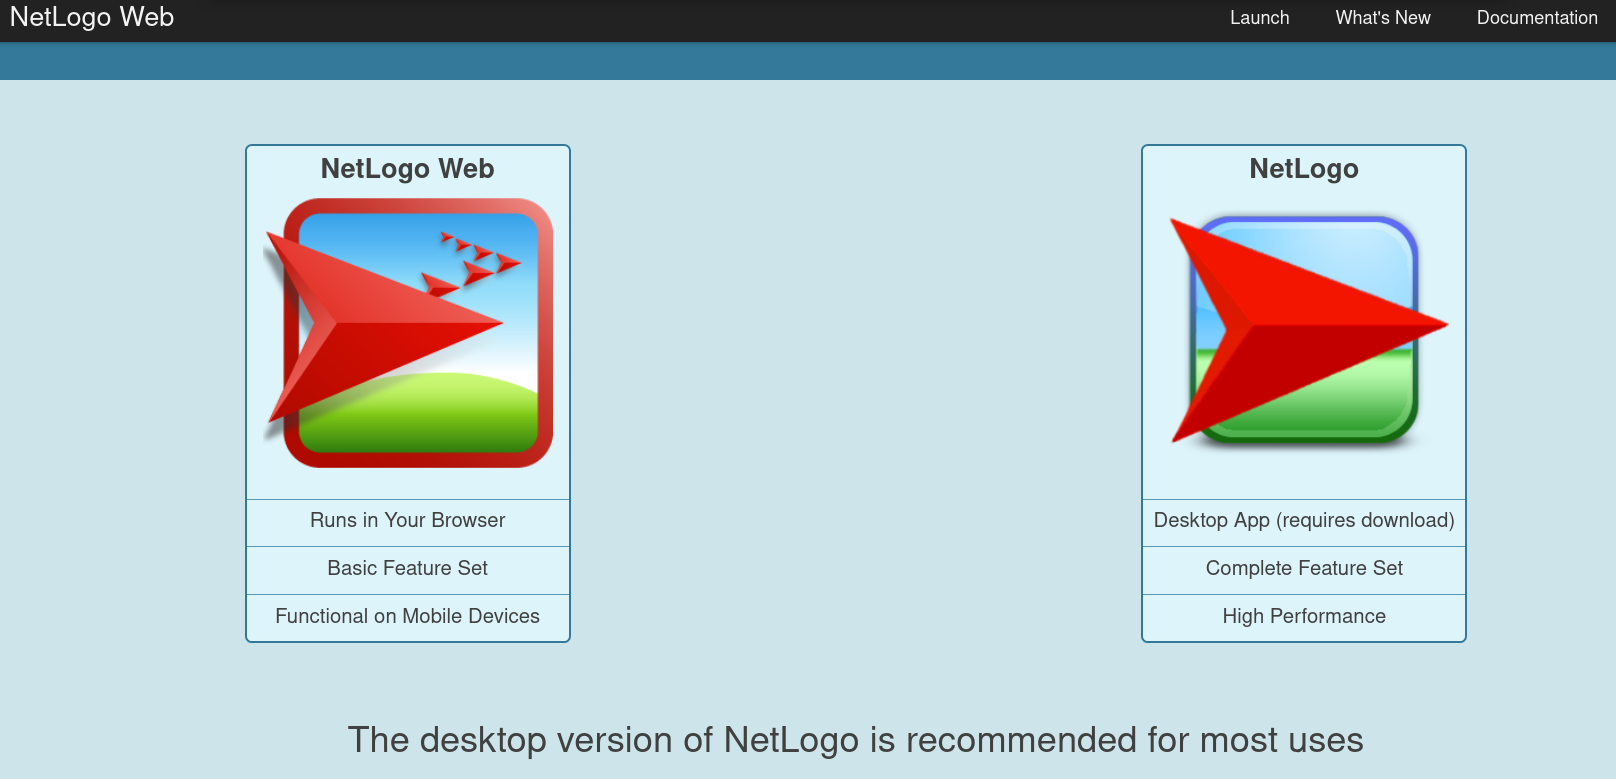
\includegraphics[width=.7\textwidth]{netlogoWeb.png}
\end{figure}      
\end{frame}

\section{NetLogo Web}
\begin{frame}
\Huge
\centering
\texttt{NetLogo Web} \\
Tutorial para su uso docente\\
\end{frame}


\begin{frame}{NetLogo Web: Paso 1}
Ingresamos a NetLogo Web
\begin{figure}
\centering
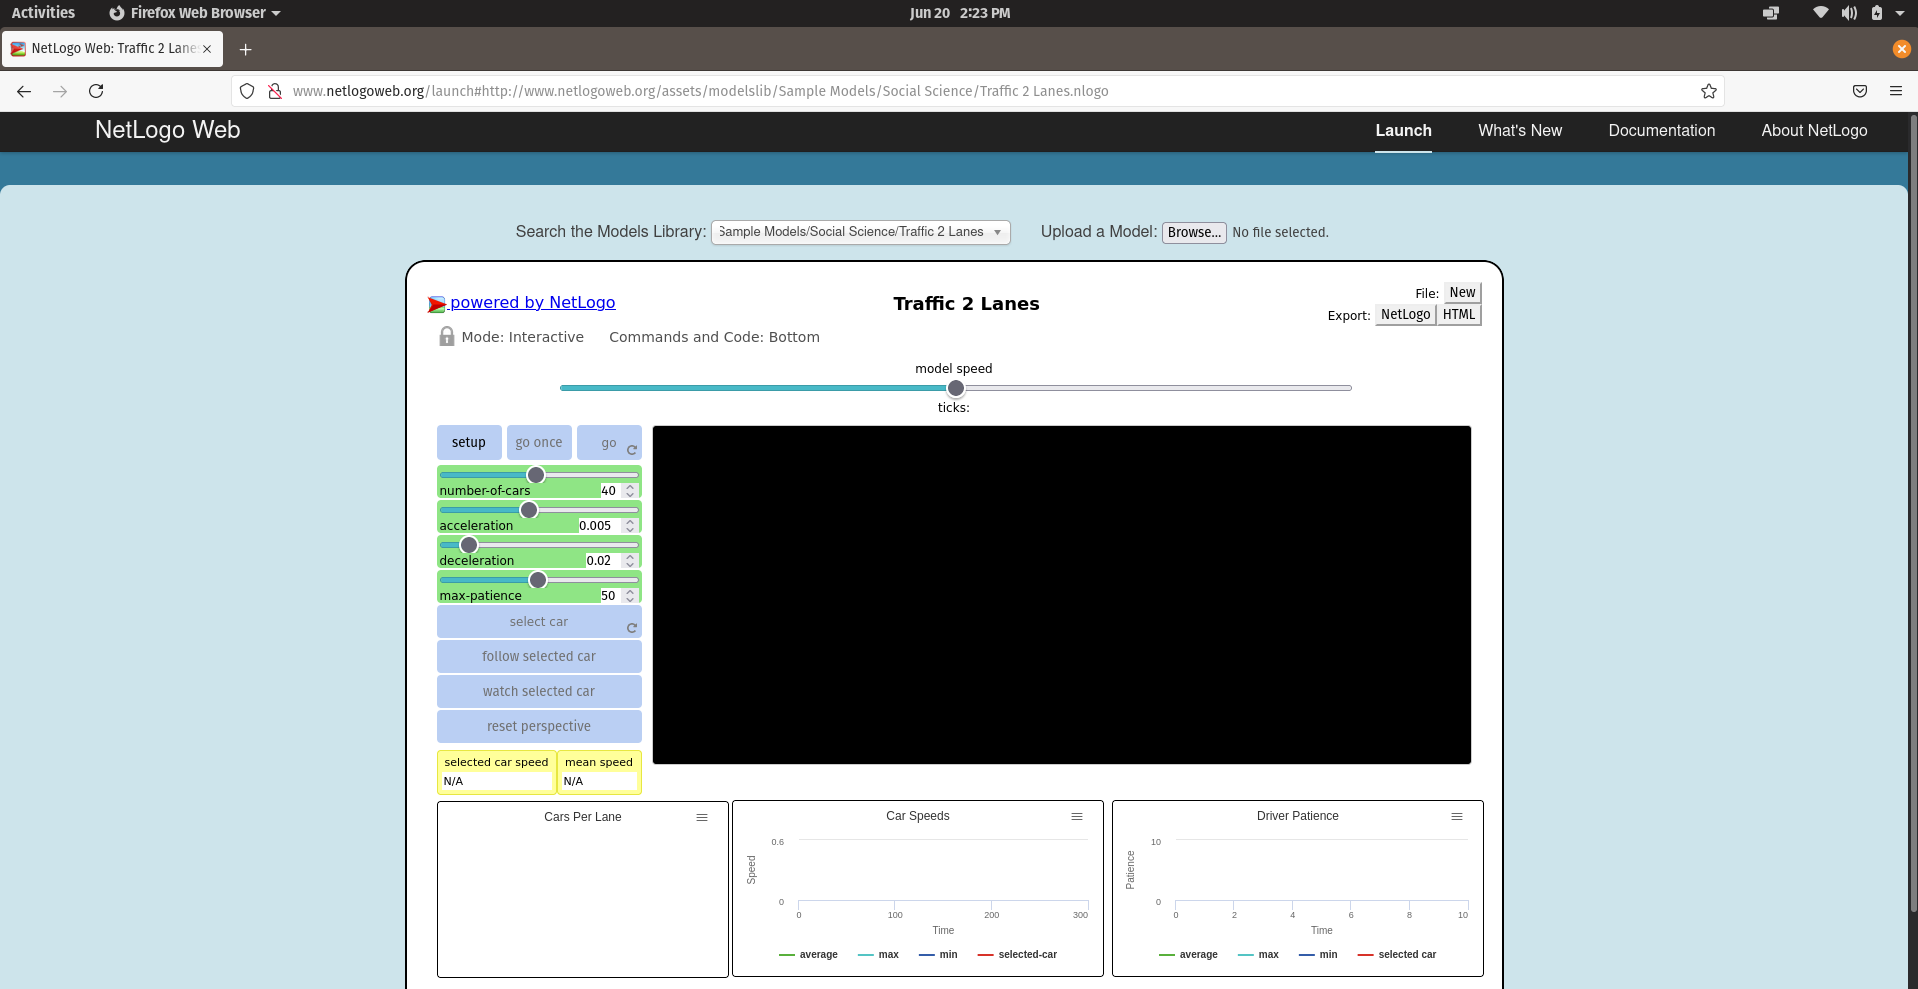
\includegraphics[width=.95\textwidth]{NetLogoWebA.png}
\end{figure}  
\end{frame}

\begin{frame}{NetLogo Web: Paso 2}
Clic en el botón Setup
\begin{figure}
\centering
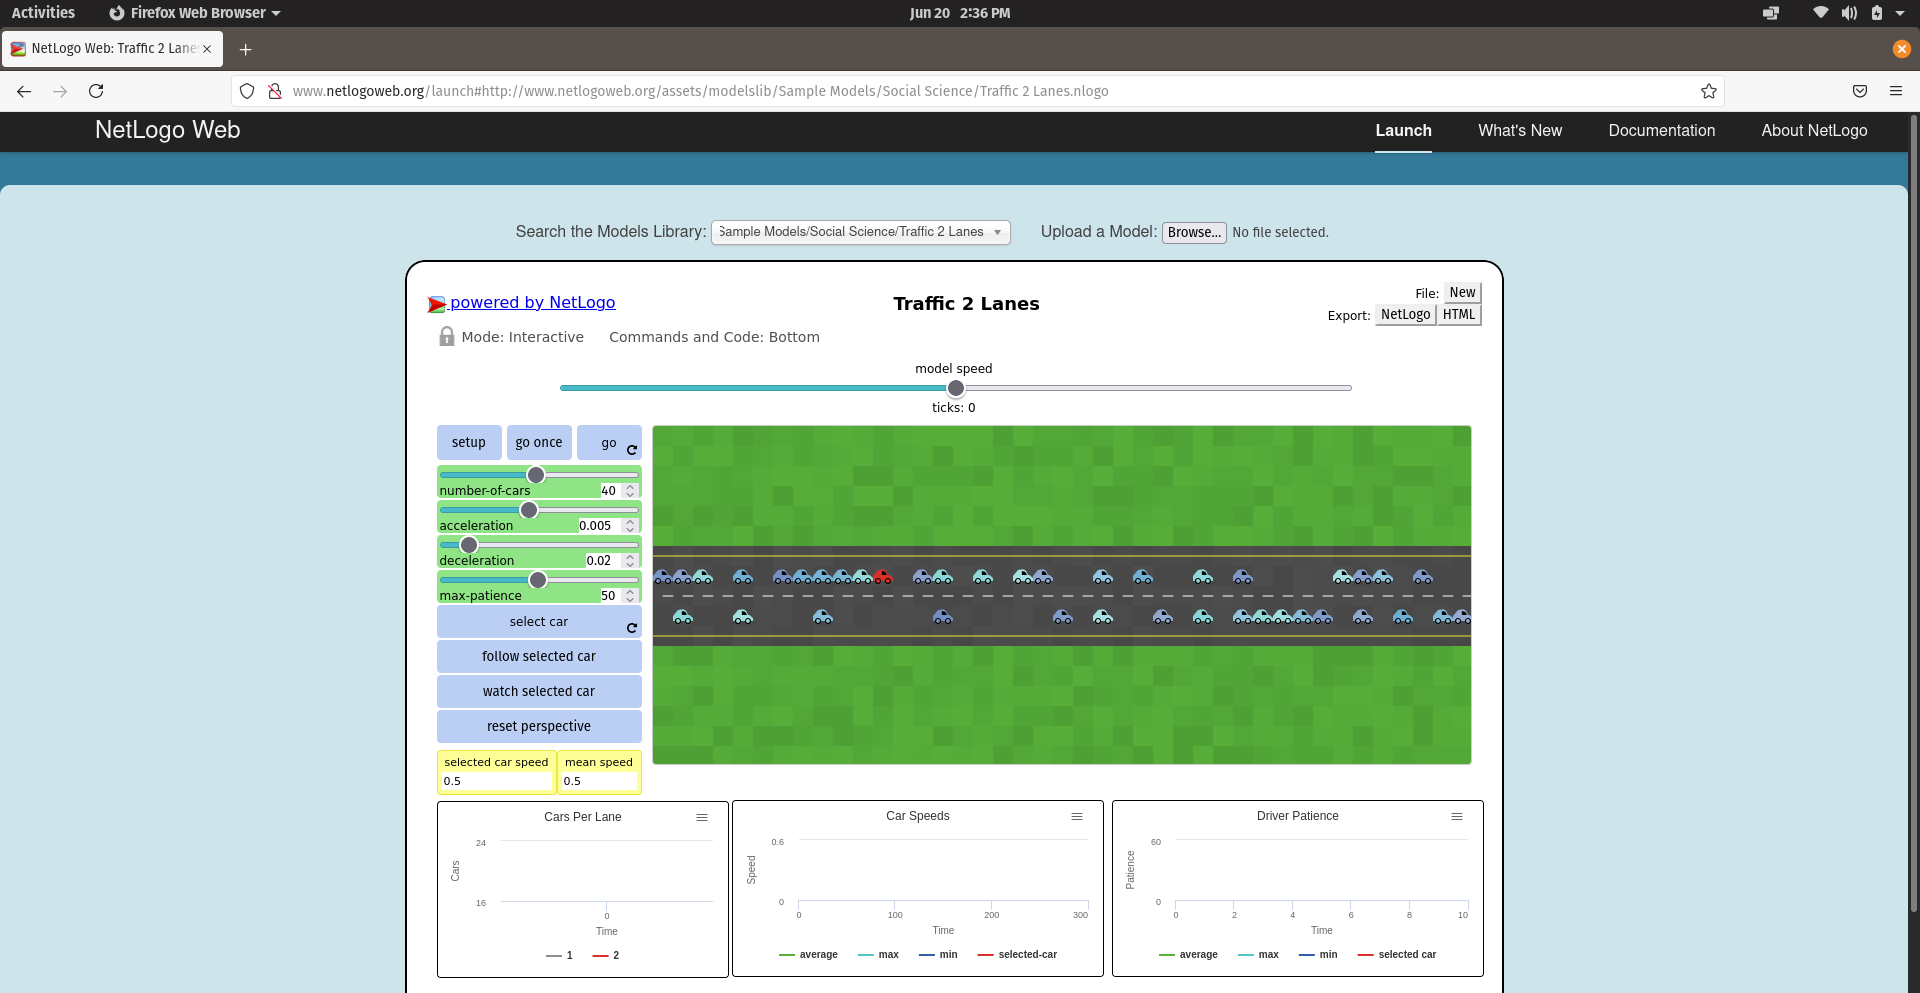
\includegraphics[width=.92\textwidth]{NetLogoWB.png}
\end{figure}  
\end{frame}

\begin{frame}{NetLogo Web: Paso 3}
Clic en el botón go
\begin{figure}
\centering
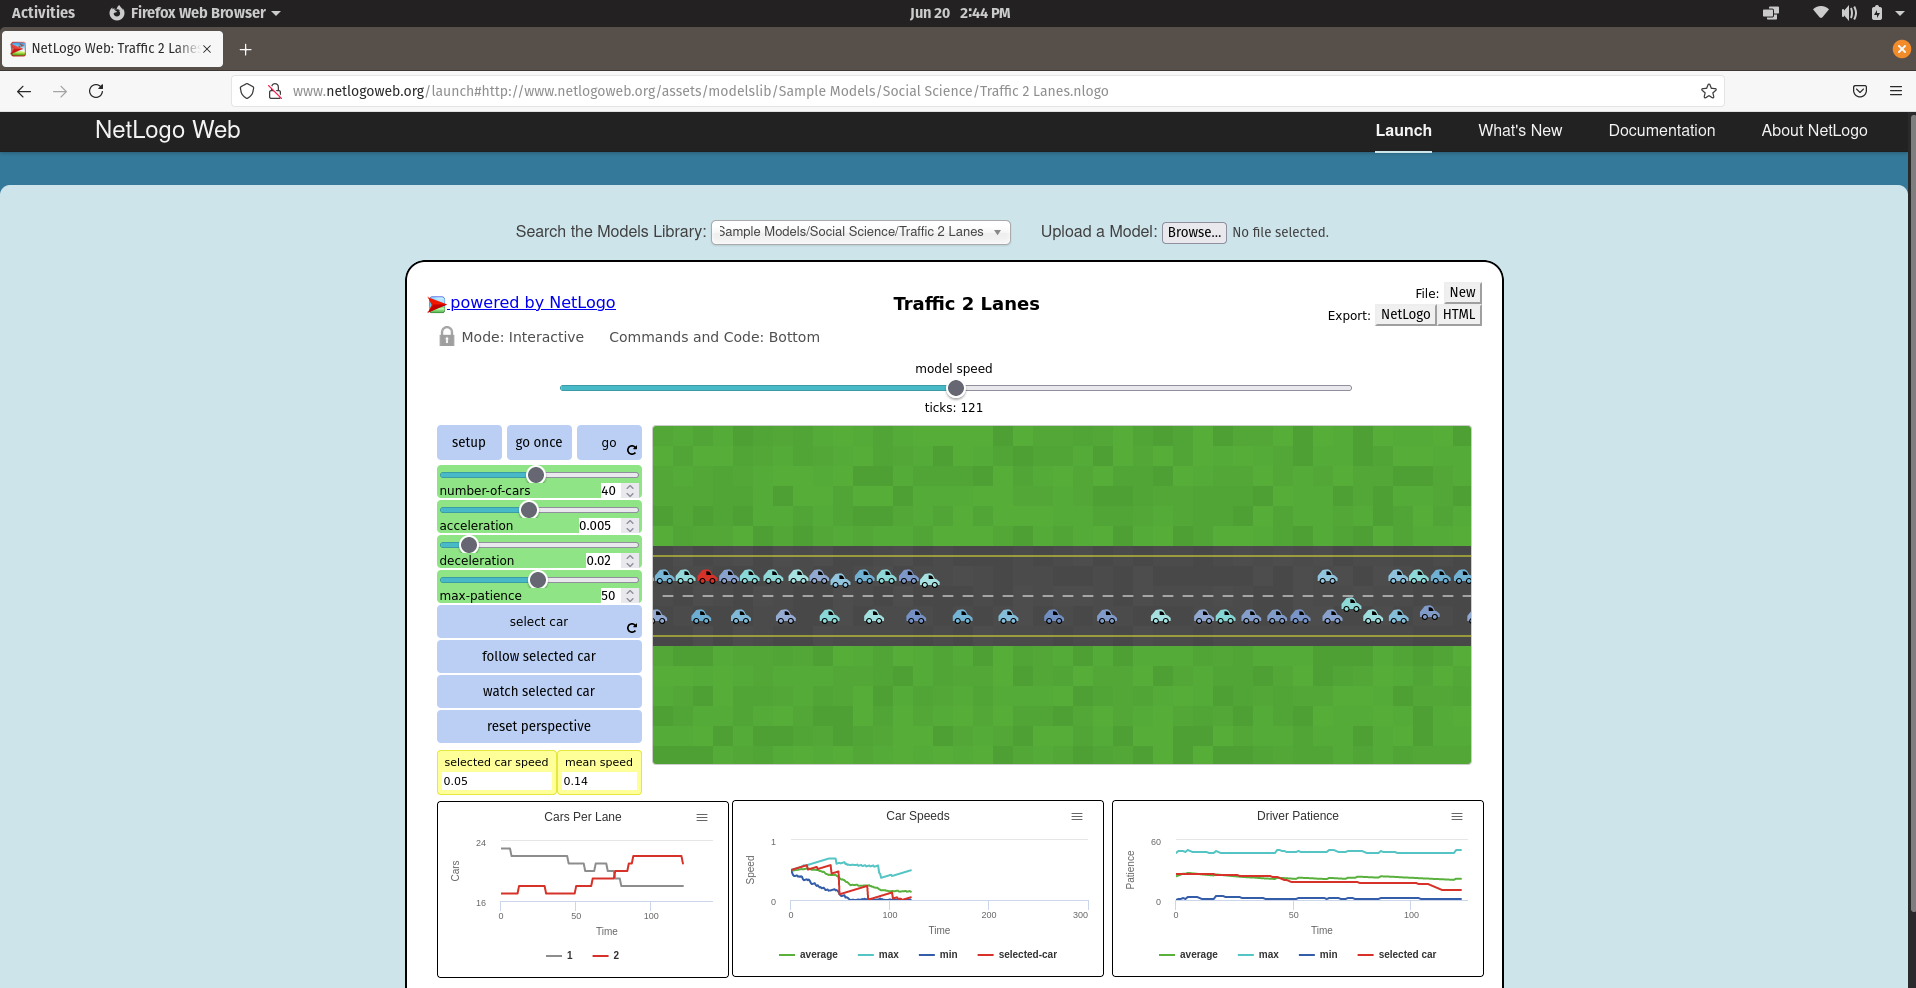
\includegraphics[width=.92\textwidth]{NetLogoWC.png}
\end{figure}  
\end{frame}

\begin{frame}{NetLogo Web: Paso 4}
Lea la información del modelo (qué es, cómo usarlo, cosas por observar, cosas por intentar, extensión del modelo).
\begin{figure}
\centering
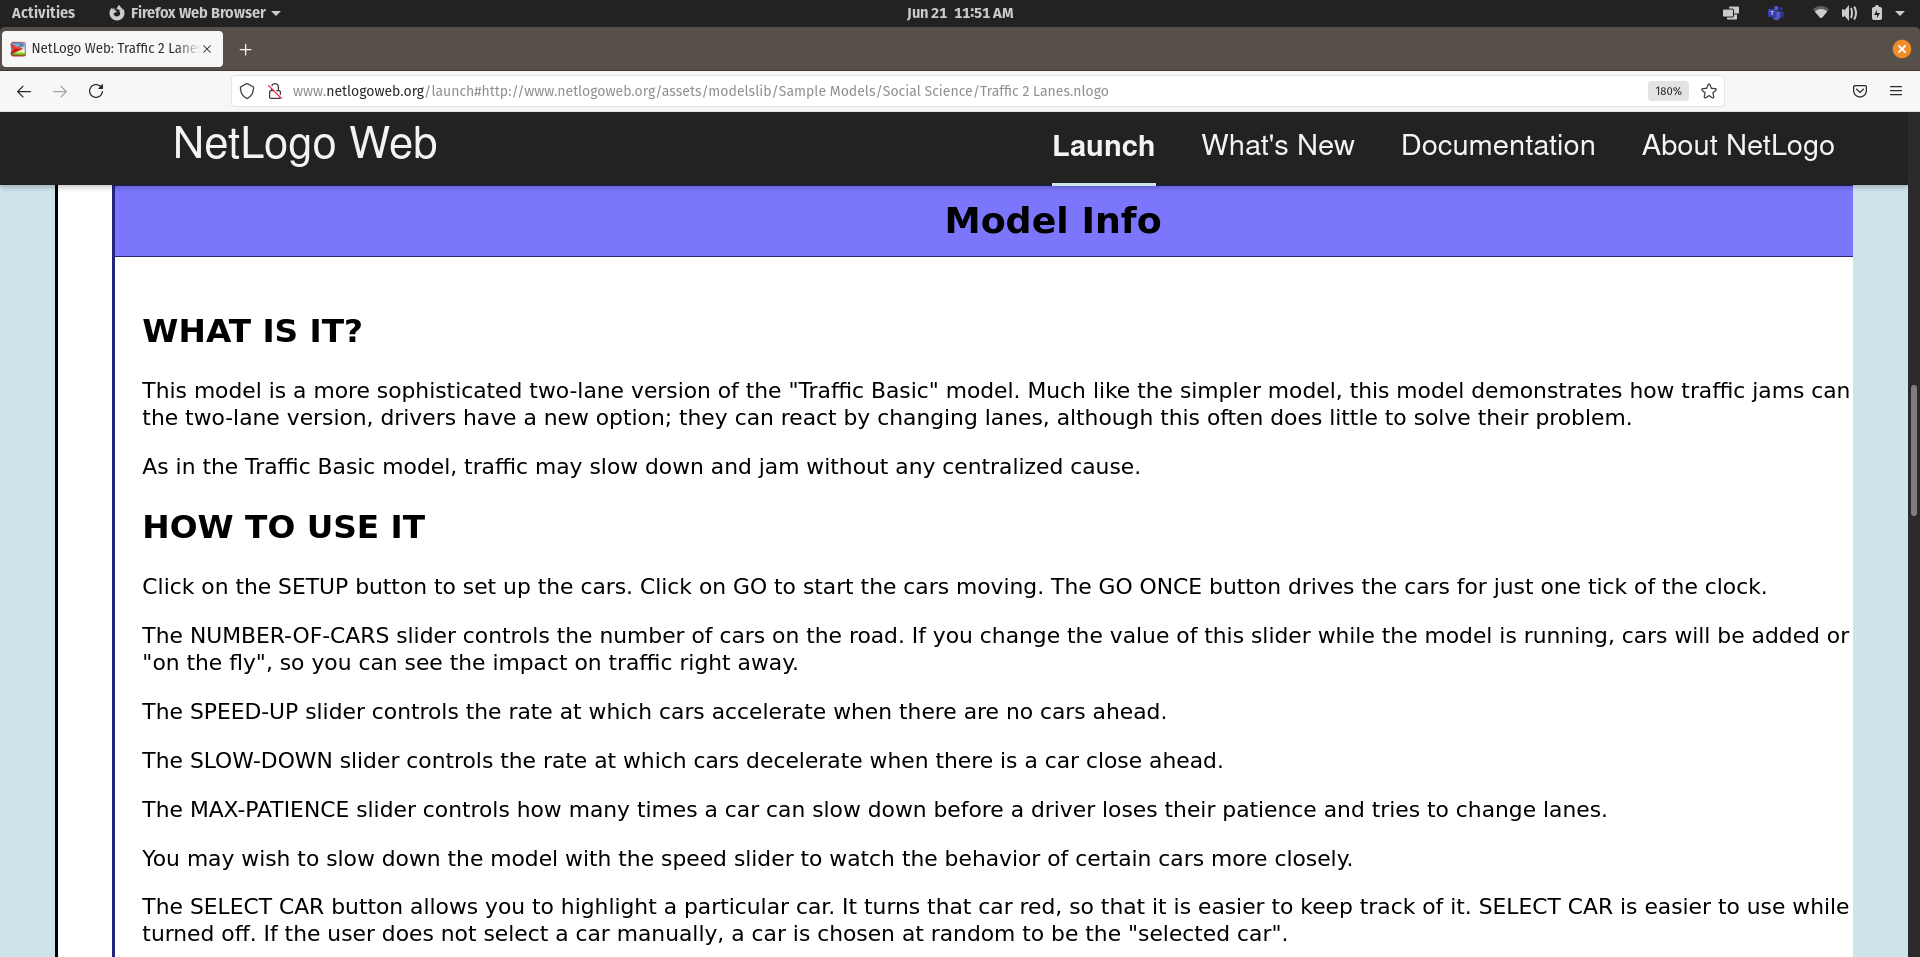
\includegraphics[width=.92\textwidth]{NetlogoC.png}
\end{figure}  
\end{frame}

\begin{frame}{NetLogo Web: Paso 5}
Explore otros modelos
\begin{figure}
\centering
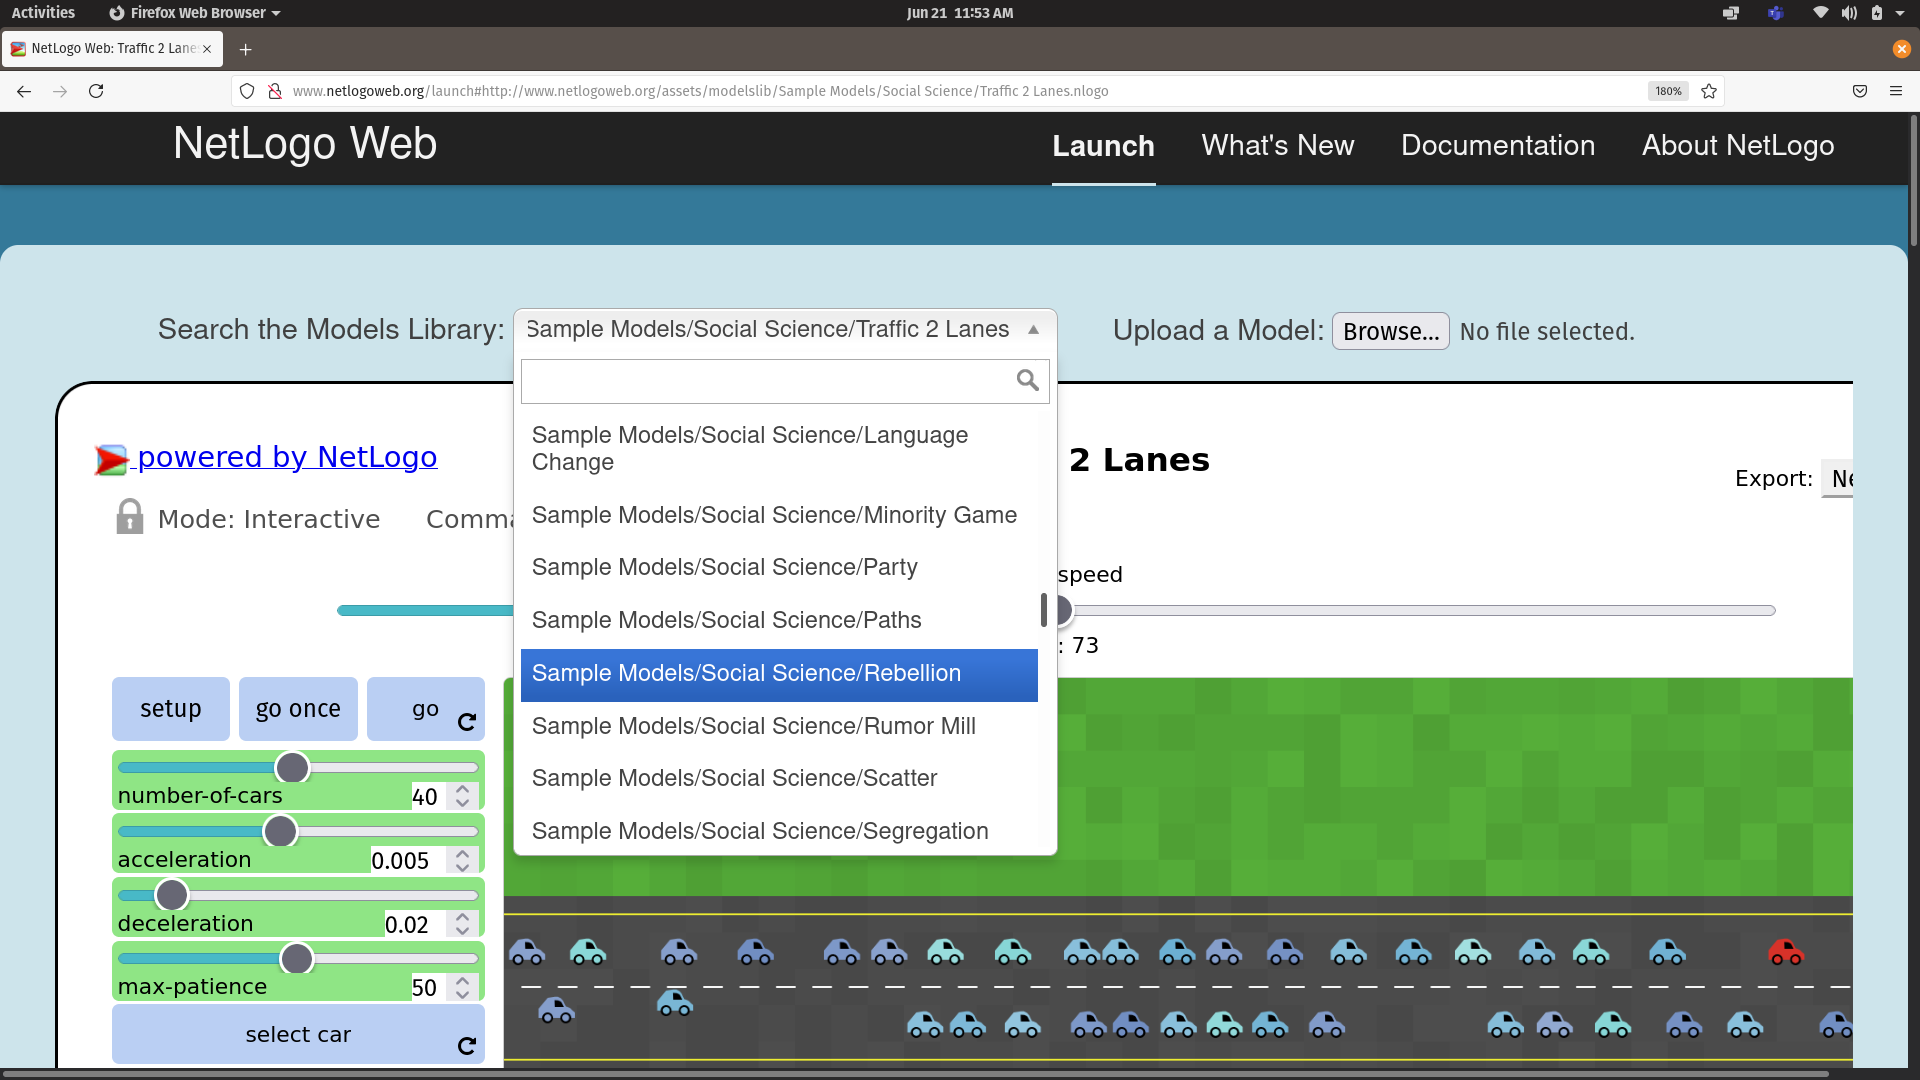
\includegraphics[width=.92\textwidth]{NetlogoD.png}
\end{figure}  
\end{frame}

\begin{frame}{NetLogo Web: Paso 6}
Explore el modelo de la caja de Galton para explicar el concepto de distribución estadística.
\begin{figure}
\centering
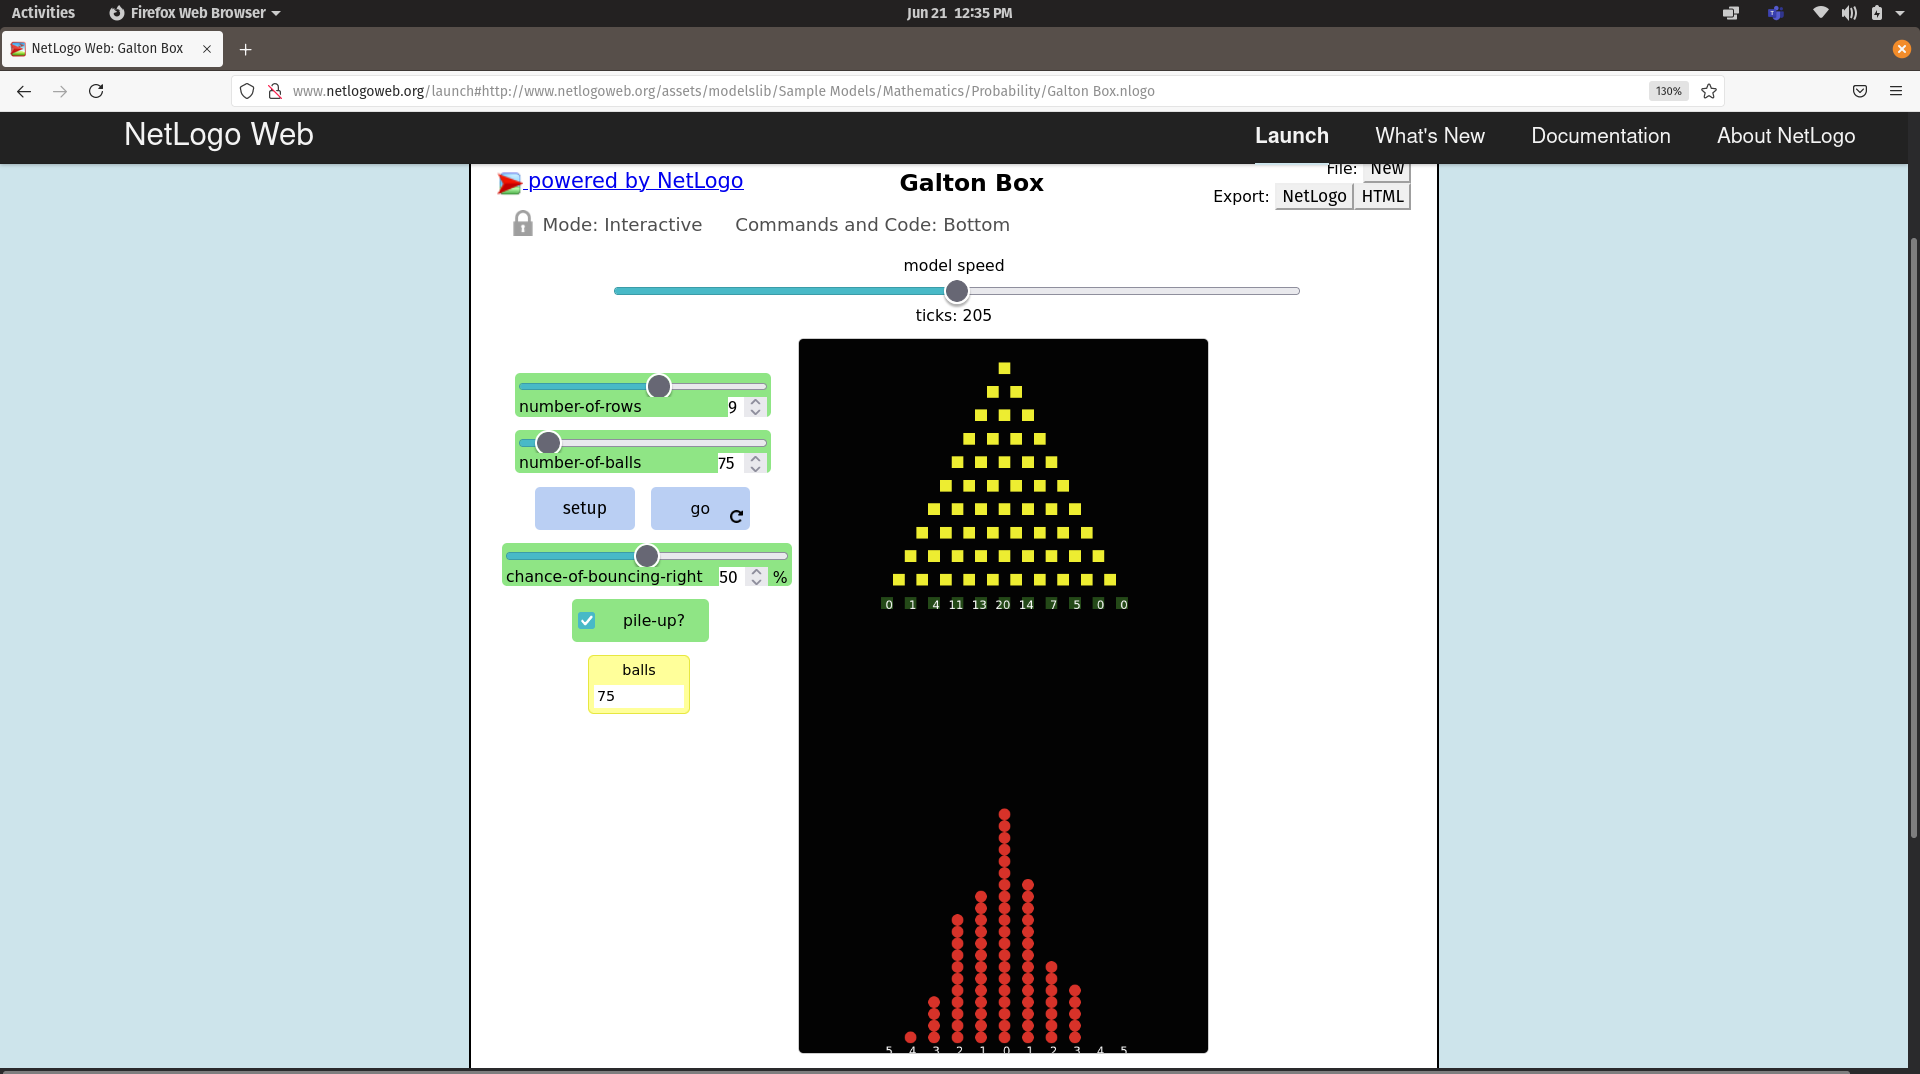
\includegraphics[width=.92\textwidth]{GaltonBox.png}
\end{figure}  
\end{frame}


\section{NetLogo en Psicología y Ciencias Sociales}
\begin{frame}{NetLogo en Psicología y Ciencias Sociales}
En psicología clínica se ha usado para comprender la estructura de la psicopatología.
\begin{figure}
\centering

\includegraphics[width=.85\textwidth]{Network.png}
\end{figure}
\cite{Borsboom2013} \textcolor{blue}{\url{https://youtu.be/AIaBkAwLd4Q}}
\end{frame}

\begin{frame}{NetLogo en Psicología y Ciencias Sociales}
En finanzas NetLogo ha servido para entender algunos aspectos asociados con el financiamiento de hogares.
\begin{figure}
\centering
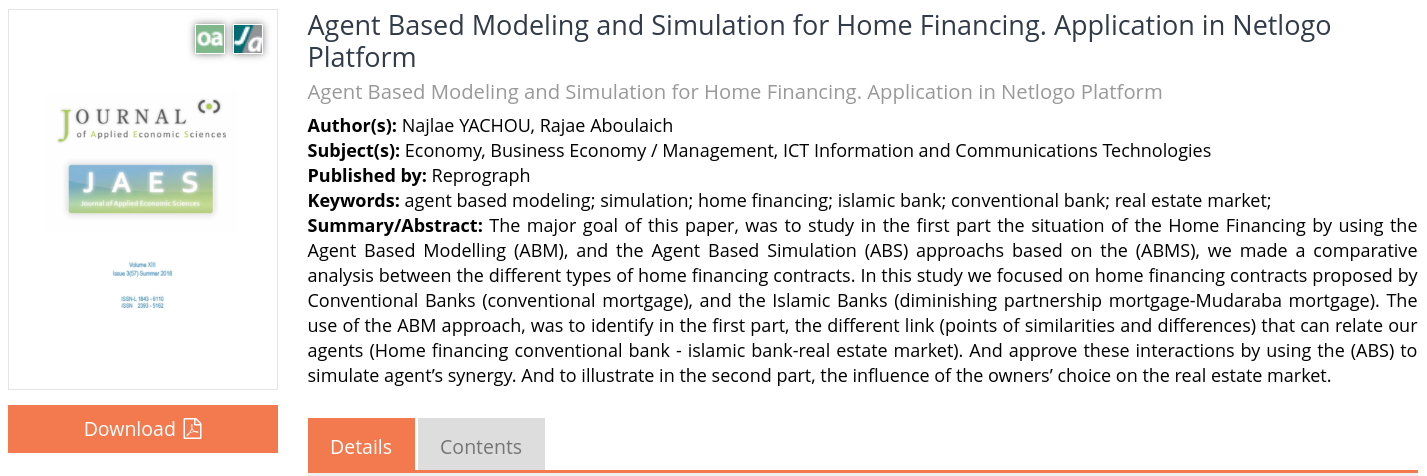
\includegraphics[width=.85\textwidth]{jaes.png}
\end{figure}  
\cite{Yachou2018}
\end{frame}

\begin{frame}{NetLogo en Psicología y Ciencias Sociales}
NetLogo se ha usado también para entender la propagación de información falsa en redes sociales.
\begin{figure}
\centering
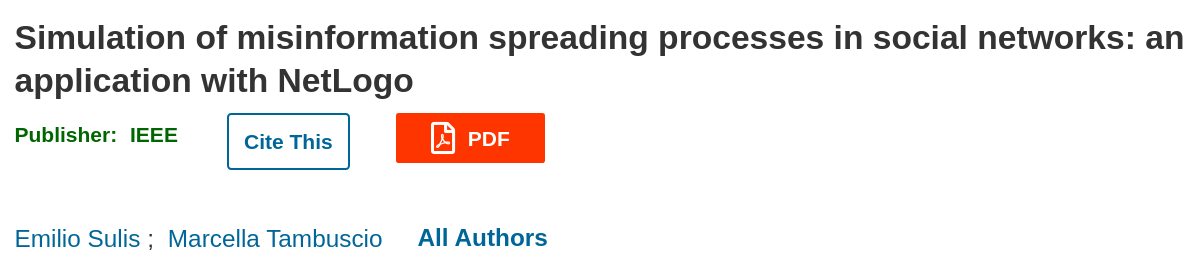
\includegraphics[width=.85\textwidth]{misinfo.png}
\end{figure}  
\cite{Sulis2020}
\end{frame}

\section{Recomendaciones}
\begin{frame}{Recomendaciones}
Explorar los recursos de la Sociedad Internacional para las Ciencias del Aprendizaje
\begin{figure}
\centering

\includegraphics[width=.85\textwidth]{ISLS.png}
\end{figure}     
\end{frame}

\begin{frame}{Recomendaciones}
Desarrollar modelos reproducibles con NetLogo, aprovechando la diversidad de modelos ya disponibles.
\begin{figure}
\centering
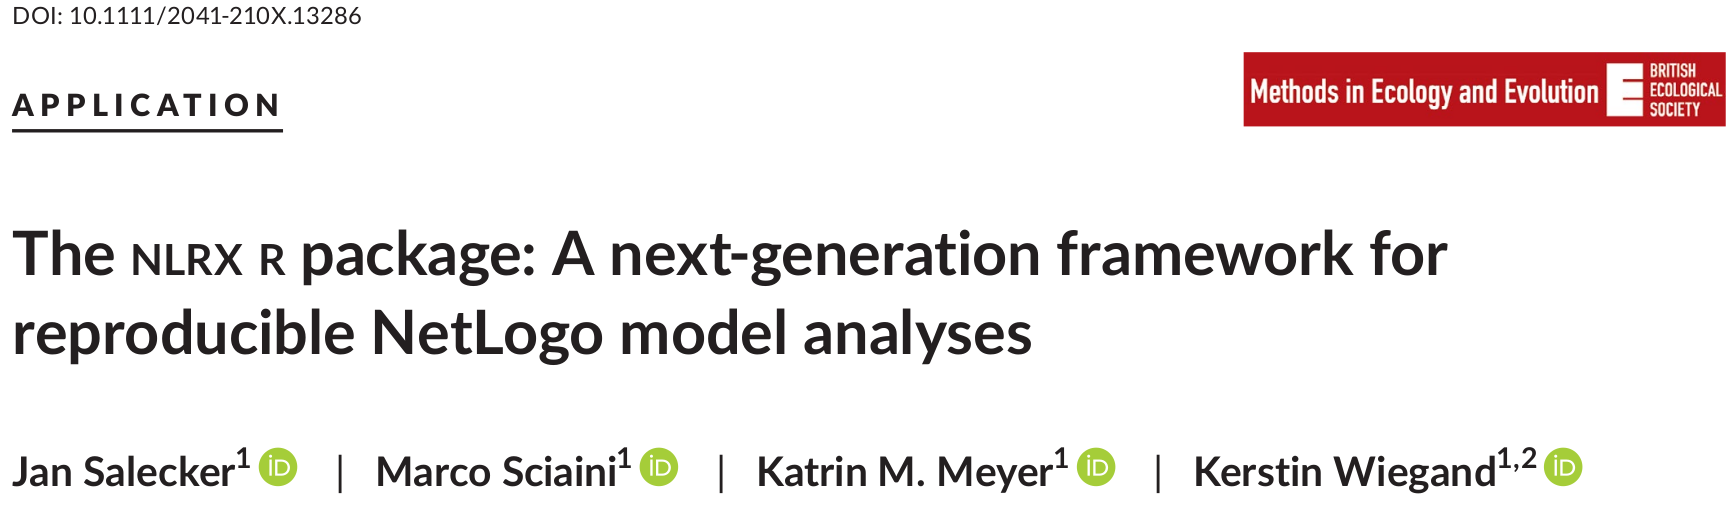
\includegraphics[width=.85\textwidth]{nlrx.png}
\end{figure}     
\cite{Salecker2019}    
\end{frame}



\begin{frame}[allowframebreaks]{Referencias}
\tiny{ 
\bibliographystyle{apacite}
\bibliography{refs}
}
\end{frame}


\end{document}